% Options for packages loaded elsewhere
\PassOptionsToPackage{unicode}{hyperref}
\PassOptionsToPackage{hyphens}{url}
%
\documentclass[
]{article}
\usepackage{amsmath,amssymb}
\usepackage{iftex}
\ifPDFTeX
  \usepackage[T1]{fontenc}
  \usepackage[utf8]{inputenc}
  \usepackage{textcomp} % provide euro and other symbols
\else % if luatex or xetex
  \usepackage{unicode-math} % this also loads fontspec
  \defaultfontfeatures{Scale=MatchLowercase}
  \defaultfontfeatures[\rmfamily]{Ligatures=TeX,Scale=1}
\fi
\usepackage{lmodern}
\ifPDFTeX\else
  % xetex/luatex font selection
\fi
% Use upquote if available, for straight quotes in verbatim environments
\IfFileExists{upquote.sty}{\usepackage{upquote}}{}
\IfFileExists{microtype.sty}{% use microtype if available
  \usepackage[]{microtype}
  \UseMicrotypeSet[protrusion]{basicmath} % disable protrusion for tt fonts
}{}
\makeatletter
\@ifundefined{KOMAClassName}{% if non-KOMA class
  \IfFileExists{parskip.sty}{%
    \usepackage{parskip}
  }{% else
    \setlength{\parindent}{0pt}
    \setlength{\parskip}{6pt plus 2pt minus 1pt}}
}{% if KOMA class
  \KOMAoptions{parskip=half}}
\makeatother
\usepackage{xcolor}
\usepackage[margin=1in]{geometry}
\usepackage{color}
\usepackage{fancyvrb}
\newcommand{\VerbBar}{|}
\newcommand{\VERB}{\Verb[commandchars=\\\{\}]}
\DefineVerbatimEnvironment{Highlighting}{Verbatim}{commandchars=\\\{\}}
% Add ',fontsize=\small' for more characters per line
\usepackage{framed}
\definecolor{shadecolor}{RGB}{248,248,248}
\newenvironment{Shaded}{\begin{snugshade}}{\end{snugshade}}
\newcommand{\AlertTok}[1]{\textcolor[rgb]{0.94,0.16,0.16}{#1}}
\newcommand{\AnnotationTok}[1]{\textcolor[rgb]{0.56,0.35,0.01}{\textbf{\textit{#1}}}}
\newcommand{\AttributeTok}[1]{\textcolor[rgb]{0.13,0.29,0.53}{#1}}
\newcommand{\BaseNTok}[1]{\textcolor[rgb]{0.00,0.00,0.81}{#1}}
\newcommand{\BuiltInTok}[1]{#1}
\newcommand{\CharTok}[1]{\textcolor[rgb]{0.31,0.60,0.02}{#1}}
\newcommand{\CommentTok}[1]{\textcolor[rgb]{0.56,0.35,0.01}{\textit{#1}}}
\newcommand{\CommentVarTok}[1]{\textcolor[rgb]{0.56,0.35,0.01}{\textbf{\textit{#1}}}}
\newcommand{\ConstantTok}[1]{\textcolor[rgb]{0.56,0.35,0.01}{#1}}
\newcommand{\ControlFlowTok}[1]{\textcolor[rgb]{0.13,0.29,0.53}{\textbf{#1}}}
\newcommand{\DataTypeTok}[1]{\textcolor[rgb]{0.13,0.29,0.53}{#1}}
\newcommand{\DecValTok}[1]{\textcolor[rgb]{0.00,0.00,0.81}{#1}}
\newcommand{\DocumentationTok}[1]{\textcolor[rgb]{0.56,0.35,0.01}{\textbf{\textit{#1}}}}
\newcommand{\ErrorTok}[1]{\textcolor[rgb]{0.64,0.00,0.00}{\textbf{#1}}}
\newcommand{\ExtensionTok}[1]{#1}
\newcommand{\FloatTok}[1]{\textcolor[rgb]{0.00,0.00,0.81}{#1}}
\newcommand{\FunctionTok}[1]{\textcolor[rgb]{0.13,0.29,0.53}{\textbf{#1}}}
\newcommand{\ImportTok}[1]{#1}
\newcommand{\InformationTok}[1]{\textcolor[rgb]{0.56,0.35,0.01}{\textbf{\textit{#1}}}}
\newcommand{\KeywordTok}[1]{\textcolor[rgb]{0.13,0.29,0.53}{\textbf{#1}}}
\newcommand{\NormalTok}[1]{#1}
\newcommand{\OperatorTok}[1]{\textcolor[rgb]{0.81,0.36,0.00}{\textbf{#1}}}
\newcommand{\OtherTok}[1]{\textcolor[rgb]{0.56,0.35,0.01}{#1}}
\newcommand{\PreprocessorTok}[1]{\textcolor[rgb]{0.56,0.35,0.01}{\textit{#1}}}
\newcommand{\RegionMarkerTok}[1]{#1}
\newcommand{\SpecialCharTok}[1]{\textcolor[rgb]{0.81,0.36,0.00}{\textbf{#1}}}
\newcommand{\SpecialStringTok}[1]{\textcolor[rgb]{0.31,0.60,0.02}{#1}}
\newcommand{\StringTok}[1]{\textcolor[rgb]{0.31,0.60,0.02}{#1}}
\newcommand{\VariableTok}[1]{\textcolor[rgb]{0.00,0.00,0.00}{#1}}
\newcommand{\VerbatimStringTok}[1]{\textcolor[rgb]{0.31,0.60,0.02}{#1}}
\newcommand{\WarningTok}[1]{\textcolor[rgb]{0.56,0.35,0.01}{\textbf{\textit{#1}}}}
\usepackage{graphicx}
\makeatletter
\def\maxwidth{\ifdim\Gin@nat@width>\linewidth\linewidth\else\Gin@nat@width\fi}
\def\maxheight{\ifdim\Gin@nat@height>\textheight\textheight\else\Gin@nat@height\fi}
\makeatother
% Scale images if necessary, so that they will not overflow the page
% margins by default, and it is still possible to overwrite the defaults
% using explicit options in \includegraphics[width, height, ...]{}
\setkeys{Gin}{width=\maxwidth,height=\maxheight,keepaspectratio}
% Set default figure placement to htbp
\makeatletter
\def\fps@figure{htbp}
\makeatother
\setlength{\emergencystretch}{3em} % prevent overfull lines
\providecommand{\tightlist}{%
  \setlength{\itemsep}{0pt}\setlength{\parskip}{0pt}}
\setcounter{secnumdepth}{-\maxdimen} % remove section numbering
\ifLuaTeX
  \usepackage{selnolig}  % disable illegal ligatures
\fi
\IfFileExists{bookmark.sty}{\usepackage{bookmark}}{\usepackage{hyperref}}
\IfFileExists{xurl.sty}{\usepackage{xurl}}{} % add URL line breaks if available
\urlstyle{same}
\hypersetup{
  pdftitle={LEARN SIMPLE R IMPLIMENTATIONS ON DATA WITH THE TITANIC DATA SET},
  pdfauthor={MUTHAMA KELVIN MUTUKU},
  hidelinks,
  pdfcreator={LaTeX via pandoc}}

\title{LEARN SIMPLE R IMPLIMENTATIONS ON DATA WITH THE TITANIC DATA SET}
\author{MUTHAMA KELVIN MUTUKU}
\date{2024-07-02}

\begin{document}
\maketitle

{
\setcounter{tocdepth}{2}
\tableofcontents
}
\hypertarget{what-is-expected-of-the-learner.}{%
\subsection{WHAT IS EXPECTED OF THE
LEARNER.}\label{what-is-expected-of-the-learner.}}

At the end of the study the learner should be able to:

\begin{enumerate}
\def\labelenumi{\arabic{enumi}.}
\tightlist
\item
  Call data in csv form.

  \begin{itemize}
  \tightlist
  \item
    view the data set.
  \item
    show and explain the structure of a given data set.
  \end{itemize}
\item
  Restore all variables to their required data types.
\item
  Draw insights from the data set given.
\item
  Visualize the data and draw insights in various plots.
\item
  model data accordingly; fitting the data to the correct model.
\end{enumerate}

\hypertarget{lets-begin.}{%
\subsection{lets begin.}\label{lets-begin.}}

In this study we will use the \textbf{TIRANIC DATA SET}. The Titanic
dataset, often used for machine learning and data analysis projects,
typically includes various attributes about the passengers and details
about their journey. The most commonly used version is available on
Kaggle, and it usually includes the following columns:

\begin{enumerate}
\def\labelenumi{\arabic{enumi}.}
\tightlist
\item
  \textbf{PassengerId}: Unique identifier for each passenger.
\item
  \textbf{Survived}: Survival status (0 = No, 1 = Yes).
\item
  \textbf{Pclass}: Ticket class (1 = 1st, 2 = 2nd, 3 = 3rd).
\item
  \textbf{Name}: Passenger's name.
\item
  \textbf{Sex}: Gender of the passenger.
\item
  \textbf{Age}: Age of the passenger.
\item
  \textbf{SibSp}: Number of siblings or spouses aboard the Titanic.
\item
  \textbf{Parch}: Number of parents or children aboard the Titanic.
\item
  \textbf{Ticket}: Ticket number.
\item
  \textbf{Fare}: Fare paid for the ticket.
\item
  \textbf{Cabin}: Cabin number (if available).
\item
  \textbf{Embarked}: Port of embarkation (C = Cherbourg, Q = Queenstown,
  S = Southampton).
\end{enumerate}

This data set allows for various types of analyses and modeling, such as
predicting survival, exploring correlations, and performing feature
engineering. Is there a specific ana lysis or task you have in mind with
the Titanic dataset?

\hypertarget{predicting-survival-classification-task}{%
\subsubsection{1. Predicting Survival (Classification
Task)}\label{predicting-survival-classification-task}}

\begin{itemize}
\tightlist
\item
  \textbf{Goal}: Build a model to predict whether a passenger survived
  or not.
\item
  \textbf{Expected Result}: A classification model (e.g., logistic
  regression, decision tree, random forest, etc.) with performance
  metrics such as accuracy, precision, recall, and F1-score. An accuracy
  around 70-80\% is often considered reasonable for this dataset.
\end{itemize}

\hypertarget{data-exploration-and-visualization}{%
\subsubsection{2. Data Exploration and
Visualization}\label{data-exploration-and-visualization}}

\begin{itemize}
\tightlist
\item
  \textbf{Goal}: Understand the dataset through exploratory data
  analysis (EDA).
\item
  \textbf{Expected Result}: Insights and visualizations such as:

  \begin{itemize}
  \tightlist
  \item
    Distribution of passengers by class, gender, and age.
  \item
    Survival rates by different features (e.g., gender, class, age).
  \item
    Correlations between different features and survival.
  \end{itemize}
\end{itemize}

\hypertarget{feature-engineering}{%
\subsubsection{3. Feature Engineering}\label{feature-engineering}}

\begin{itemize}
\tightlist
\item
  \textbf{Goal}: Create new features that could improve model
  performance.
\item
  \textbf{Expected Result}: New features such as:

  \begin{itemize}
  \tightlist
  \item
    Family size (combining SibSp and Parch).
  \item
    Title extracted from the Name column.
  \item
    Age group bins.
  \item
    Fare per person (Fare divided by the number of people in the same
    ticket).
  \end{itemize}
\end{itemize}

\hypertarget{model-evaluation-and-comparison}{%
\subsubsection{4. Model Evaluation and
Comparison}\label{model-evaluation-and-comparison}}

\begin{itemize}
\tightlist
\item
  \textbf{Goal}: Compare different models to find the best performing
  one.
\item
  \textbf{Expected Result}: Performance metrics (accuracy, precision,
  recall, F1-score, ROC-AUC) for different models and a discussion of
  the best model based on these metrics.
\end{itemize}

\hypertarget{deployment}{%
\subsubsection{5. Deployment}\label{deployment}}

\begin{itemize}
\tightlist
\item
  \textbf{Goal}: Deploy the model for practical use.
\item
  \textbf{Expected Result}: A deployed model that can take new passenger
  data as input and predict the survival outcome. This could be done
  using a web application, API, or other means.
\end{itemize}

\hypertarget{example-workflow}{%
\subsubsection{Example Workflow:}\label{example-workflow}}

\begin{enumerate}
\def\labelenumi{\arabic{enumi}.}
\tightlist
\item
  \textbf{Data Cleaning}: Handle missing values, correct data types,
  etc.
\item
  \textbf{EDA}: Visualize and summarize key patterns and relationships.
\item
  \textbf{Feature Engineering}: Create and select features that improve
  model performance.
\item
  \textbf{Model Building}: Train various models and tune
  hyperparameters.
\item
  \textbf{Model Evaluation}: Compare models and select the best one.
\item
  \textbf{Conclusion}: Summarize findings and insights.
\end{enumerate}

\hypertarget{calling-the-required-libraries.}{%
\subsection{Calling the required
libraries.}\label{calling-the-required-libraries.}}

\begin{Shaded}
\begin{Highlighting}[]
\FunctionTok{library}\NormalTok{(}\StringTok{"dplyr"}\NormalTok{)}
\end{Highlighting}
\end{Shaded}

\begin{verbatim}
## 
## Attaching package: 'dplyr'
\end{verbatim}

\begin{verbatim}
## The following objects are masked from 'package:stats':
## 
##     filter, lag
\end{verbatim}

\begin{verbatim}
## The following objects are masked from 'package:base':
## 
##     intersect, setdiff, setequal, union
\end{verbatim}

\begin{Shaded}
\begin{Highlighting}[]
\FunctionTok{library}\NormalTok{(}\StringTok{"datasets"}\NormalTok{)}
\FunctionTok{library}\NormalTok{(}\StringTok{"ggplot2"}\NormalTok{)}
\FunctionTok{library}\NormalTok{(}\StringTok{"graphics"}\NormalTok{)}
\FunctionTok{library}\NormalTok{(}\StringTok{"stats"}\NormalTok{)}
\FunctionTok{library}\NormalTok{(}\StringTok{"ggeffects"}\NormalTok{)}
\FunctionTok{library}\NormalTok{(}\StringTok{"randomForest"}\NormalTok{)}
\end{Highlighting}
\end{Shaded}

\begin{verbatim}
## randomForest 4.7-1.1
\end{verbatim}

\begin{verbatim}
## Type rfNews() to see new features/changes/bug fixes.
\end{verbatim}

\begin{verbatim}
## 
## Attaching package: 'randomForest'
\end{verbatim}

\begin{verbatim}
## The following object is masked from 'package:ggplot2':
## 
##     margin
\end{verbatim}

\begin{verbatim}
## The following object is masked from 'package:dplyr':
## 
##     combine
\end{verbatim}

\hypertarget{creating-the-dataframes.}{%
\subsection{creating the dataframes.}\label{creating-the-dataframes.}}

\begin{Shaded}
\begin{Highlighting}[]
\CommentTok{\#calling the dataset}
\NormalTok{titanic\_train\_data }\OtherTok{\textless{}{-}} \FunctionTok{read.csv}\NormalTok{(}\StringTok{\textquotesingle{}C:/Users/EliteBook/OneDrive/Desktop/DATA SCIENCE PERSONAL PROJECTS/TITANIC/train.csv\textquotesingle{}}\NormalTok{)}
\NormalTok{titanic\_test\_data }\OtherTok{\textless{}{-}} \FunctionTok{read.csv}\NormalTok{(}\StringTok{\textquotesingle{}C:/Users/EliteBook/OneDrive/Desktop/DATA SCIENCE PERSONAL PROJECTS/TITANIC/test.csv\textquotesingle{}}\NormalTok{)}
\end{Highlighting}
\end{Shaded}

We can have a view of the datasets for some clear understanding and
knowledge of the workflow.

\begin{Shaded}
\begin{Highlighting}[]
\CommentTok{\#viewing the dataset}
\FunctionTok{head}\NormalTok{(titanic\_train\_data)}
\end{Highlighting}
\end{Shaded}

\begin{verbatim}
##   PassengerId Survived Pclass
## 1           1        0      3
## 2           2        1      1
## 3           3        1      3
## 4           4        1      1
## 5           5        0      3
## 6           6        0      3
##                                                  Name    Sex Age SibSp Parch
## 1                             Braund, Mr. Owen Harris   male  22     1     0
## 2 Cumings, Mrs. John Bradley (Florence Briggs Thayer) female  38     1     0
## 3                              Heikkinen, Miss. Laina female  26     0     0
## 4        Futrelle, Mrs. Jacques Heath (Lily May Peel) female  35     1     0
## 5                            Allen, Mr. William Henry   male  35     0     0
## 6                                    Moran, Mr. James   male  NA     0     0
##             Ticket    Fare Cabin Embarked
## 1        A/5 21171  7.2500              S
## 2         PC 17599 71.2833   C85        C
## 3 STON/O2. 3101282  7.9250              S
## 4           113803 53.1000  C123        S
## 5           373450  8.0500              S
## 6           330877  8.4583              Q
\end{verbatim}

\begin{Shaded}
\begin{Highlighting}[]
\FunctionTok{head}\NormalTok{(titanic\_test\_data)}
\end{Highlighting}
\end{Shaded}

\begin{verbatim}
##   PassengerId Pclass                                         Name    Sex  Age
## 1         892      3                             Kelly, Mr. James   male 34.5
## 2         893      3             Wilkes, Mrs. James (Ellen Needs) female 47.0
## 3         894      2                    Myles, Mr. Thomas Francis   male 62.0
## 4         895      3                             Wirz, Mr. Albert   male 27.0
## 5         896      3 Hirvonen, Mrs. Alexander (Helga E Lindqvist) female 22.0
## 6         897      3                   Svensson, Mr. Johan Cervin   male 14.0
##   SibSp Parch  Ticket    Fare Cabin Embarked
## 1     0     0  330911  7.8292              Q
## 2     1     0  363272  7.0000              S
## 3     0     0  240276  9.6875              Q
## 4     0     0  315154  8.6625              S
## 5     1     1 3101298 12.2875              S
## 6     0     0    7538  9.2250              S
\end{verbatim}

Viewing the data gives you a general look on what you are dealin with
but with the help of \textbf{str()} you can clearly understand the
datta's structure.

\begin{Shaded}
\begin{Highlighting}[]
\FunctionTok{str}\NormalTok{(titanic\_train\_data)}
\end{Highlighting}
\end{Shaded}

\begin{verbatim}
## 'data.frame':    891 obs. of  12 variables:
##  $ PassengerId: int  1 2 3 4 5 6 7 8 9 10 ...
##  $ Survived   : int  0 1 1 1 0 0 0 0 1 1 ...
##  $ Pclass     : int  3 1 3 1 3 3 1 3 3 2 ...
##  $ Name       : chr  "Braund, Mr. Owen Harris" "Cumings, Mrs. John Bradley (Florence Briggs Thayer)" "Heikkinen, Miss. Laina" "Futrelle, Mrs. Jacques Heath (Lily May Peel)" ...
##  $ Sex        : chr  "male" "female" "female" "female" ...
##  $ Age        : num  22 38 26 35 35 NA 54 2 27 14 ...
##  $ SibSp      : int  1 1 0 1 0 0 0 3 0 1 ...
##  $ Parch      : int  0 0 0 0 0 0 0 1 2 0 ...
##  $ Ticket     : chr  "A/5 21171" "PC 17599" "STON/O2. 3101282" "113803" ...
##  $ Fare       : num  7.25 71.28 7.92 53.1 8.05 ...
##  $ Cabin      : chr  "" "C85" "" "C123" ...
##  $ Embarked   : chr  "S" "C" "S" "S" ...
\end{verbatim}

You can now tell some essential features of the data according to:

\begin{itemize}
\tightlist
\item
  The dimensions (891 rows and 12 columns).
\item
  The data types (int:integer, chr:character, num:numeric).
\end{itemize}

\begin{Shaded}
\begin{Highlighting}[]
\FunctionTok{str}\NormalTok{(titanic\_test\_data)}
\end{Highlighting}
\end{Shaded}

\begin{verbatim}
## 'data.frame':    418 obs. of  11 variables:
##  $ PassengerId: int  892 893 894 895 896 897 898 899 900 901 ...
##  $ Pclass     : int  3 3 2 3 3 3 3 2 3 3 ...
##  $ Name       : chr  "Kelly, Mr. James" "Wilkes, Mrs. James (Ellen Needs)" "Myles, Mr. Thomas Francis" "Wirz, Mr. Albert" ...
##  $ Sex        : chr  "male" "female" "male" "male" ...
##  $ Age        : num  34.5 47 62 27 22 14 30 26 18 21 ...
##  $ SibSp      : int  0 1 0 0 1 0 0 1 0 2 ...
##  $ Parch      : int  0 0 0 0 1 0 0 1 0 0 ...
##  $ Ticket     : chr  "330911" "363272" "240276" "315154" ...
##  $ Fare       : num  7.83 7 9.69 8.66 12.29 ...
##  $ Cabin      : chr  "" "" "" "" ...
##  $ Embarked   : chr  "Q" "S" "Q" "S" ...
\end{verbatim}

Same to the \textbf{titanic\_test\_data} you also can now tell some
essential features of the data according to:

\begin{itemize}
\tightlist
\item
  The dimensions (891 rows and 11 columns),
\item
  The data types (int:integer, chr:character, num:numeric).
\end{itemize}

In addition you can use the \textbf{summary()} function to tell features
of the dataset.

\begin{Shaded}
\begin{Highlighting}[]
\FunctionTok{summary}\NormalTok{(titanic\_train\_data)}
\end{Highlighting}
\end{Shaded}

\begin{verbatim}
##   PassengerId       Survived          Pclass          Name          
##  Min.   :  1.0   Min.   :0.0000   Min.   :1.000   Length:891        
##  1st Qu.:223.5   1st Qu.:0.0000   1st Qu.:2.000   Class :character  
##  Median :446.0   Median :0.0000   Median :3.000   Mode  :character  
##  Mean   :446.0   Mean   :0.3838   Mean   :2.309                     
##  3rd Qu.:668.5   3rd Qu.:1.0000   3rd Qu.:3.000                     
##  Max.   :891.0   Max.   :1.0000   Max.   :3.000                     
##                                                                     
##      Sex                 Age            SibSp           Parch       
##  Length:891         Min.   : 0.42   Min.   :0.000   Min.   :0.0000  
##  Class :character   1st Qu.:20.12   1st Qu.:0.000   1st Qu.:0.0000  
##  Mode  :character   Median :28.00   Median :0.000   Median :0.0000  
##                     Mean   :29.70   Mean   :0.523   Mean   :0.3816  
##                     3rd Qu.:38.00   3rd Qu.:1.000   3rd Qu.:0.0000  
##                     Max.   :80.00   Max.   :8.000   Max.   :6.0000  
##                     NA's   :177                                     
##     Ticket               Fare           Cabin             Embarked        
##  Length:891         Min.   :  0.00   Length:891         Length:891        
##  Class :character   1st Qu.:  7.91   Class :character   Class :character  
##  Mode  :character   Median : 14.45   Mode  :character   Mode  :character  
##                     Mean   : 32.20                                        
##                     3rd Qu.: 31.00                                        
##                     Max.   :512.33                                        
## 
\end{verbatim}

\begin{Shaded}
\begin{Highlighting}[]
\FunctionTok{summary}\NormalTok{(titanic\_test\_data)}
\end{Highlighting}
\end{Shaded}

\begin{verbatim}
##   PassengerId         Pclass          Name               Sex           
##  Min.   : 892.0   Min.   :1.000   Length:418         Length:418        
##  1st Qu.: 996.2   1st Qu.:1.000   Class :character   Class :character  
##  Median :1100.5   Median :3.000   Mode  :character   Mode  :character  
##  Mean   :1100.5   Mean   :2.266                                        
##  3rd Qu.:1204.8   3rd Qu.:3.000                                        
##  Max.   :1309.0   Max.   :3.000                                        
##                                                                        
##       Age            SibSp            Parch           Ticket         
##  Min.   : 0.17   Min.   :0.0000   Min.   :0.0000   Length:418        
##  1st Qu.:21.00   1st Qu.:0.0000   1st Qu.:0.0000   Class :character  
##  Median :27.00   Median :0.0000   Median :0.0000   Mode  :character  
##  Mean   :30.27   Mean   :0.4474   Mean   :0.3923                     
##  3rd Qu.:39.00   3rd Qu.:1.0000   3rd Qu.:0.0000                     
##  Max.   :76.00   Max.   :8.0000   Max.   :9.0000                     
##  NA's   :86                                                          
##       Fare            Cabin             Embarked        
##  Min.   :  0.000   Length:418         Length:418        
##  1st Qu.:  7.896   Class :character   Class :character  
##  Median : 14.454   Mode  :character   Mode  :character  
##  Mean   : 35.627                                        
##  3rd Qu.: 31.500                                        
##  Max.   :512.329                                        
##  NA's   :1
\end{verbatim}

With the help of this function we can check the:

\begin{itemize}
\tightlist
\item
  length of a given column(variable).
\item
  Measure of spread of the data:

  \begin{itemize}
  \tightlist
  \item
    Mean.
  \item
    Median.
  \item
    Quantiles.
  \item
    Range.
  \item
    min.
  \item
    max.
  \end{itemize}
\end{itemize}

\hypertarget{cleaning-the-data.}{%
\subsection{Cleaning the data.}\label{cleaning-the-data.}}

In this process we will have to concider variables with: - missinng
values. - outliers. - Wrong datatypes.

\hypertarget{transforming-the-data-with-levels-to-factor.}{%
\subsubsection{1. Transforming the data with levels to
factor.}\label{transforming-the-data-with-levels-to-factor.}}

Using the \textbf{as.factor()} function we can convert a variable to
bieng in levles. eg:

The \textbf{Pclass} has three levels which are:

\begin{itemize}
\tightlist
\item
  class 1
\item
  class 2
\item
  class 3
\end{itemize}

\begin{Shaded}
\begin{Highlighting}[]
\CommentTok{\#setting factors to categorical data}
\NormalTok{titanic\_train\_data}\SpecialCharTok{$}\NormalTok{Pclass}\OtherTok{\textless{}{-}}\FunctionTok{as.factor}\NormalTok{(titanic\_train\_data}\SpecialCharTok{$}\NormalTok{Pclass)}
\NormalTok{titanic\_train\_data}\SpecialCharTok{$}\NormalTok{Embarked}\OtherTok{\textless{}{-}}\FunctionTok{as.factor}\NormalTok{(titanic\_train\_data}\SpecialCharTok{$}\NormalTok{Embarked)}
\NormalTok{titanic\_train\_data}\SpecialCharTok{$}\NormalTok{Sex}\OtherTok{\textless{}{-}}\FunctionTok{as.factor}\NormalTok{(titanic\_train\_data}\SpecialCharTok{$}\NormalTok{Sex)}

\NormalTok{titanic\_test\_data}\SpecialCharTok{$}\NormalTok{Pclass}\OtherTok{\textless{}{-}}\FunctionTok{as.factor}\NormalTok{(titanic\_test\_data}\SpecialCharTok{$}\NormalTok{Pclass)}
\NormalTok{titanic\_test\_data}\SpecialCharTok{$}\NormalTok{Embarked}\OtherTok{\textless{}{-}}\FunctionTok{as.factor}\NormalTok{(titanic\_test\_data}\SpecialCharTok{$}\NormalTok{Embarked)}
\NormalTok{titanic\_test\_data}\SpecialCharTok{$}\NormalTok{Sex}\OtherTok{\textless{}{-}}\FunctionTok{as.factor}\NormalTok{(titanic\_test\_data}\SpecialCharTok{$}\NormalTok{Sex)}
\end{Highlighting}
\end{Shaded}

If you were to call the \textbf{str()} of the data you will see that the
type of some variables has changed to factor.

\begin{Shaded}
\begin{Highlighting}[]
\FunctionTok{str}\NormalTok{(titanic\_train\_data)}
\end{Highlighting}
\end{Shaded}

\begin{verbatim}
## 'data.frame':    891 obs. of  12 variables:
##  $ PassengerId: int  1 2 3 4 5 6 7 8 9 10 ...
##  $ Survived   : int  0 1 1 1 0 0 0 0 1 1 ...
##  $ Pclass     : Factor w/ 3 levels "1","2","3": 3 1 3 1 3 3 1 3 3 2 ...
##  $ Name       : chr  "Braund, Mr. Owen Harris" "Cumings, Mrs. John Bradley (Florence Briggs Thayer)" "Heikkinen, Miss. Laina" "Futrelle, Mrs. Jacques Heath (Lily May Peel)" ...
##  $ Sex        : Factor w/ 2 levels "female","male": 2 1 1 1 2 2 2 2 1 1 ...
##  $ Age        : num  22 38 26 35 35 NA 54 2 27 14 ...
##  $ SibSp      : int  1 1 0 1 0 0 0 3 0 1 ...
##  $ Parch      : int  0 0 0 0 0 0 0 1 2 0 ...
##  $ Ticket     : chr  "A/5 21171" "PC 17599" "STON/O2. 3101282" "113803" ...
##  $ Fare       : num  7.25 71.28 7.92 53.1 8.05 ...
##  $ Cabin      : chr  "" "C85" "" "C123" ...
##  $ Embarked   : Factor w/ 4 levels "","C","Q","S": 4 2 4 4 4 3 4 4 4 2 ...
\end{verbatim}

You will notice that even though the \textbf{survived} varible in
\textbf{titanic\_train\_data} has two levels(0 and 1), we have not
factored it. This is because we will use it for some analysis and errors
call if it is factored.

\hypertarget{missing-values.}{%
\subsubsection{2. missing values.}\label{missing-values.}}

For the missing values there various ways of dealing with them, you can
choose to:

\begin{itemize}
\tightlist
\item
  Ignore the missing values.
\item
  Impute the missing values.
\item
  Remove the missing values.
\end{itemize}

All this depends on the dataset you are working on and the insights you
need from the data.

\hypertarget{identifying-the-missing-values.}{%
\paragraph{Identifying the missing
values.}\label{identifying-the-missing-values.}}

We will first check for missing values in all the variables.

\begin{Shaded}
\begin{Highlighting}[]
\NormalTok{titanic\_train\_data }\SpecialCharTok{\%\textgreater{}\%}
  \FunctionTok{is.na}\NormalTok{() }\SpecialCharTok{\%\textgreater{}\%}
  \FunctionTok{table}\NormalTok{()}
\end{Highlighting}
\end{Shaded}

\begin{verbatim}
## .
## FALSE  TRUE 
## 10515   177
\end{verbatim}

We can see that we have 177 null values, but we can't tell their
specific variables. To do so we can;

\begin{Shaded}
\begin{Highlighting}[]
\FunctionTok{filter\_all}\NormalTok{(titanic\_train\_data, }\FunctionTok{any\_vars}\NormalTok{(}\FunctionTok{is.na}\NormalTok{(.))) }\SpecialCharTok{\%\textgreater{}\%}
  \FunctionTok{head}\NormalTok{()}
\end{Highlighting}
\end{Shaded}

\begin{verbatim}
##   PassengerId Survived Pclass                          Name    Sex Age SibSp
## 1           6        0      3              Moran, Mr. James   male  NA     0
## 2          18        1      2  Williams, Mr. Charles Eugene   male  NA     0
## 3          20        1      3       Masselmani, Mrs. Fatima female  NA     0
## 4          27        0      3       Emir, Mr. Farred Chehab   male  NA     0
## 5          29        1      3 O'Dwyer, Miss. Ellen "Nellie" female  NA     0
## 6          30        0      3           Todoroff, Mr. Lalio   male  NA     0
##   Parch Ticket    Fare Cabin Embarked
## 1     0 330877  8.4583              Q
## 2     0 244373 13.0000              S
## 3     0   2649  7.2250              C
## 4     0   2631  7.2250              C
## 5     0 330959  7.8792              Q
## 6     0 349216  7.8958              S
\end{verbatim}

According to our data the only variable with null values is the
\textbf{Age} variable. It contains 177 null values.

In addition there is a varable with \textbf{empty characters}, and this
is the \textbf{embarked} variable.

\begin{Shaded}
\begin{Highlighting}[]
\NormalTok{titanic\_train\_data}\SpecialCharTok{$}\NormalTok{Embarked }\SpecialCharTok{\%\textgreater{}\%}
  \FunctionTok{table}\NormalTok{()}
\end{Highlighting}
\end{Shaded}

\begin{verbatim}
## .
##       C   Q   S 
##   2 168  77 644
\end{verbatim}

According to our data there are two values that have empty characters.

\hypertarget{dealing-with-the-missing-values.}{%
\paragraph{dealing with the missing
values.}\label{dealing-with-the-missing-values.}}

We will impute our data(fill the data using mean, median or mode). Most
precisely we will have to use the mean of the data.

Lets begin with variable \textbf{Age}.

\begin{Shaded}
\begin{Highlighting}[]
\CommentTok{\#calculating the mean.}
\NormalTok{mean.titanic\_train\_data}\OtherTok{\textless{}{-}} \FunctionTok{mean}\NormalTok{(titanic\_train\_data}\SpecialCharTok{$}\NormalTok{Age, }\AttributeTok{na.rm =}\NormalTok{ T)}

\CommentTok{\#Imputing the data.}
\NormalTok{titanic\_train\_data}\SpecialCharTok{$}\NormalTok{Age}\OtherTok{\textless{}{-}}\NormalTok{ titanic\_train\_data}\SpecialCharTok{\%\textgreater{}\%}
  \FunctionTok{select}\NormalTok{(Age) }\SpecialCharTok{\%\textgreater{}\%}
  \FunctionTok{apply}\NormalTok{(}\FunctionTok{c}\NormalTok{(}\DecValTok{2}\NormalTok{), . }\SpecialCharTok{\%\textgreater{}\%}\NormalTok{ \{}\FunctionTok{ifelse}\NormalTok{(}\FunctionTok{is.na}\NormalTok{(.), mean.titanic\_train\_data, .)\})}
\NormalTok{titanic\_test\_data}\SpecialCharTok{$}\NormalTok{Age}\OtherTok{\textless{}{-}}\NormalTok{ titanic\_test\_data}\SpecialCharTok{\%\textgreater{}\%}
  \FunctionTok{select}\NormalTok{(Age) }\SpecialCharTok{\%\textgreater{}\%}
  \FunctionTok{apply}\NormalTok{(}\FunctionTok{c}\NormalTok{(}\DecValTok{2}\NormalTok{), . }\SpecialCharTok{\%\textgreater{}\%}\NormalTok{ \{}\FunctionTok{ifelse}\NormalTok{(}\FunctionTok{is.na}\NormalTok{(.), }\FloatTok{29.70}\NormalTok{, .)\})}
\end{Highlighting}
\end{Shaded}

Next, we can work on the missing values in \textbf{Embarked}.

\begin{Shaded}
\begin{Highlighting}[]
\NormalTok{titanic\_train\_data[titanic\_train\_data}\SpecialCharTok{$}\NormalTok{Embarked }\SpecialCharTok{==} \StringTok{\textquotesingle{}\textquotesingle{}}\NormalTok{, }\StringTok{"Embarked"}\NormalTok{] }\OtherTok{\textless{}{-}} \StringTok{\textquotesingle{}S\textquotesingle{}}

\NormalTok{titanic\_test\_data[titanic\_test\_data}\SpecialCharTok{$}\NormalTok{Embarked }\SpecialCharTok{==} \StringTok{\textquotesingle{}\textquotesingle{}}\NormalTok{, }\StringTok{"Embarked"}\NormalTok{] }\OtherTok{\textless{}{-}} \StringTok{\textquotesingle{}S\textquotesingle{}}
\end{Highlighting}
\end{Shaded}

Before concluding on the missing values, you will notice that we have
left out the missing values in \textbf{Cabin}. This is heavy duty but
you can draw your conclusions from the internet and other sources. Now
that we are done with the missing values, we can proceed to the next
part.

\hypertarget{clussering-our-data-into-understandable-and-meaningful-subgroups.}{%
\subsection{Clussering our data into understandable and meaningful
subgroups.}\label{clussering-our-data-into-understandable-and-meaningful-subgroups.}}

For better understanding of the data clustering can be done, where you
devide a variable set into small subsets. Eg: the variable \textbf{age}
is large, but we can devide it into: The elderly, Non-youth, Youth and
Children.

\begin{Shaded}
\begin{Highlighting}[]
\CommentTok{\#creating an age cluser}
\NormalTok{titanic\_train\_data}\OtherTok{\textless{}{-}}\NormalTok{ titanic\_train\_data }\SpecialCharTok{\%\textgreater{}\%}
  \FunctionTok{mutate}\NormalTok{(}\AttributeTok{age\_groups =} \FunctionTok{ifelse}\NormalTok{(}\DecValTok{0}\SpecialCharTok{\textless{}=}\NormalTok{Age }\SpecialCharTok{\&}\NormalTok{ Age}\SpecialCharTok{\textless{}=}\DecValTok{13}\NormalTok{, }\DecValTok{1}\NormalTok{, }\FunctionTok{ifelse}\NormalTok{(}\DecValTok{14}\SpecialCharTok{\textless{}=}\NormalTok{Age }\SpecialCharTok{\&}\NormalTok{ Age}\SpecialCharTok{\textless{}=}\DecValTok{35}\NormalTok{, }\DecValTok{2}\NormalTok{, }\FunctionTok{ifelse}\NormalTok{(}\DecValTok{36}\SpecialCharTok{\textless{}=}\NormalTok{Age }\SpecialCharTok{\&}\NormalTok{ Age}\SpecialCharTok{\textless{}=}\DecValTok{60}\NormalTok{, }\DecValTok{3}\NormalTok{, }\DecValTok{4}\NormalTok{))))}
\end{Highlighting}
\end{Shaded}

In the data:

\begin{itemize}
\tightlist
\item
  1 stands for children.
\item
  2 stands for youth.
\item
  3 stands for adults.
\item
  4 stands for elderly.
\end{itemize}

Other additional clusters are as follows.

\begin{Shaded}
\begin{Highlighting}[]
\CommentTok{\#Additional age clusers}
\NormalTok{titanic\_train\_data}\OtherTok{\textless{}{-}}\NormalTok{ titanic\_train\_data }\SpecialCharTok{\%\textgreater{}\%}
  \FunctionTok{mutate}\NormalTok{(}\AttributeTok{age\_groups\_young =} \FunctionTok{ifelse}\NormalTok{(}\DecValTok{0}\SpecialCharTok{\textless{}=}\NormalTok{Age }\SpecialCharTok{\&}\NormalTok{ Age}\SpecialCharTok{\textless{}=}\DecValTok{13}\NormalTok{, }\StringTok{"child"}\NormalTok{,}\FunctionTok{ifelse}\NormalTok{(}\DecValTok{13}\SpecialCharTok{\textless{}=}\NormalTok{Age }\SpecialCharTok{\&}\NormalTok{ Age}\SpecialCharTok{\textless{}=}\DecValTok{35}\NormalTok{, }\StringTok{"youth"}\NormalTok{, }\StringTok{"adult"}\NormalTok{)))}

\NormalTok{titanic\_train\_data}\OtherTok{\textless{}{-}}\NormalTok{ titanic\_train\_data }\SpecialCharTok{\%\textgreater{}\%}
  \FunctionTok{mutate}\NormalTok{(}\AttributeTok{age\_groups\_children =} \FunctionTok{ifelse}\NormalTok{(}\DecValTok{0}\SpecialCharTok{\textless{}=}\NormalTok{Age }\SpecialCharTok{\&}\NormalTok{ Age}\SpecialCharTok{\textless{}=}\DecValTok{5}\NormalTok{, }\StringTok{"infant"}\NormalTok{,}\FunctionTok{ifelse}\NormalTok{(}\DecValTok{5}\SpecialCharTok{\textless{}=}\NormalTok{Age }\SpecialCharTok{\&}\NormalTok{ Age}\SpecialCharTok{\textless{}=}\DecValTok{7}\NormalTok{, }\StringTok{"child"}\NormalTok{,}\FunctionTok{ifelse}\NormalTok{(}\DecValTok{7}\SpecialCharTok{\textless{}=}\NormalTok{Age }\SpecialCharTok{\&}\NormalTok{ Age}\SpecialCharTok{\textless{}=}\DecValTok{13}\NormalTok{, }\StringTok{"teen"}\NormalTok{, }\StringTok{"non{-}child"}\NormalTok{))))}
\end{Highlighting}
\end{Shaded}

\hypertarget{grouping-the-data-to-help-with-analysis.}{%
\subsection{Grouping the data to help with
analysis.}\label{grouping-the-data-to-help-with-analysis.}}

With the help of \textbf{groupby()} function, we can get insights from
the data as follows.

\begin{Shaded}
\begin{Highlighting}[]
\CommentTok{\#analysing the data by grouping}
\NormalTok{titanic\_train\_data}\SpecialCharTok{\%\textgreater{}\%}
  \FunctionTok{group\_by}\NormalTok{(Pclass)}\SpecialCharTok{\%\textgreater{}\%}
  \FunctionTok{summarise}\NormalTok{(}\FunctionTok{mean}\NormalTok{(Survived))}
\end{Highlighting}
\end{Shaded}

\begin{verbatim}
## # A tibble: 3 x 2
##   Pclass `mean(Survived)`
##   <fct>             <dbl>
## 1 1                 0.630
## 2 2                 0.473
## 3 3                 0.242
\end{verbatim}

using the mean we can tell chances of people surviving according to
their \textbf{Pclass}. In class one, the chances of survival were
.6296296 and those of class two were 0.4728261 while class three had
0.2423625. This interpratation is logic as we expect the first class to
be well equiped incase of any damages or accident.

\begin{Shaded}
\begin{Highlighting}[]
\NormalTok{titanic\_train\_data}\SpecialCharTok{\%\textgreater{}\%}
  \FunctionTok{group\_by}\NormalTok{(Sex)}\SpecialCharTok{\%\textgreater{}\%}
  \FunctionTok{summarise}\NormalTok{(}\FunctionTok{mean}\NormalTok{(Survived))}
\end{Highlighting}
\end{Shaded}

\begin{verbatim}
## # A tibble: 2 x 2
##   Sex    `mean(Survived)`
##   <fct>             <dbl>
## 1 female            0.742
## 2 male              0.189
\end{verbatim}

According to the analysis, the females had higher chances of surviving
than men. In the incident women were highly concidered and were offered
more saving boats than men because men were believed to swim and survive
hardships better.

\begin{Shaded}
\begin{Highlighting}[]
\NormalTok{titanic\_train\_data}\SpecialCharTok{\%\textgreater{}\%}
  \FunctionTok{group\_by}\NormalTok{(SibSp)}\SpecialCharTok{\%\textgreater{}\%}
  \FunctionTok{summarise}\NormalTok{(}\FunctionTok{mean}\NormalTok{(Survived))}
\end{Highlighting}
\end{Shaded}

\begin{verbatim}
## # A tibble: 7 x 2
##   SibSp `mean(Survived)`
##   <int>            <dbl>
## 1     0            0.345
## 2     1            0.536
## 3     2            0.464
## 4     3            0.25 
## 5     4            0.167
## 6     5            0    
## 7     8            0
\end{verbatim}

According to the analysis, it seems there were people with up to 8
siblings and that the chances of surval are not well defined but bigger
families never survived. Maybe as they tried to save each other the more
they died.

\begin{Shaded}
\begin{Highlighting}[]
\NormalTok{titanic\_train\_data}\SpecialCharTok{\%\textgreater{}\%}
  \FunctionTok{group\_by}\NormalTok{(Parch)}\SpecialCharTok{\%\textgreater{}\%}
  \FunctionTok{summarise}\NormalTok{(}\FunctionTok{mean}\NormalTok{(Survived))}
\end{Highlighting}
\end{Shaded}

\begin{verbatim}
## # A tibble: 7 x 2
##   Parch `mean(Survived)`
##   <int>            <dbl>
## 1     0            0.344
## 2     1            0.551
## 3     2            0.5  
## 4     3            0.6  
## 5     4            0    
## 6     5            0.2  
## 7     6            0
\end{verbatim}

Same as the \textbf{SibSp}, it seems there were families with up to 6
children and that the chances of surval are not well defined but bigger
families never survived. Maybe as they tried to save each other the more
they died.

\begin{Shaded}
\begin{Highlighting}[]
\NormalTok{titanic\_train\_data }\SpecialCharTok{\%\textgreater{}\%}
  \FunctionTok{group\_by}\NormalTok{(age\_groups\_children)}\SpecialCharTok{\%\textgreater{}\%}
  \FunctionTok{summarise}\NormalTok{( }\FunctionTok{mean}\NormalTok{(Survived))}
\end{Highlighting}
\end{Shaded}

\begin{verbatim}
## # A tibble: 4 x 2
##   age_groups_children[,"Age"] `mean(Survived)`
##   <chr>                                  <dbl>
## 1 child                                  0.5  
## 2 infant                                 0.705
## 3 non-child                              0.366
## 4 teen                                   0.381
\end{verbatim}

\begin{Shaded}
\begin{Highlighting}[]
\CommentTok{\#setting factors to categorical data}
\NormalTok{titanic\_train\_data}\SpecialCharTok{$}\NormalTok{Survived}\OtherTok{\textless{}{-}} \FunctionTok{as.factor}\NormalTok{(titanic\_train\_data}\SpecialCharTok{$}\NormalTok{Survived)}
\end{Highlighting}
\end{Shaded}

\hypertarget{visualising-the-data-for-insights}{%
\subsection{Visualising the data for
insights}\label{visualising-the-data-for-insights}}

In this part we will ensure that we plot variables to see their
relationships and give insights

\begin{Shaded}
\begin{Highlighting}[]
\NormalTok{titanic\_train\_data }\SpecialCharTok{\%\textgreater{}\%}
  \FunctionTok{select}\NormalTok{(Survived, Pclass,, Fare, Ticket ,age\_groups, Sex,Age) }\SpecialCharTok{\%\textgreater{}\%}
  \FunctionTok{ggplot}\NormalTok{(}\AttributeTok{data=}\NormalTok{) }\SpecialCharTok{+} 
  \FunctionTok{geom\_point}\NormalTok{(}\AttributeTok{mapping =}  \FunctionTok{aes}\NormalTok{(}\AttributeTok{x=}\NormalTok{Fare, }\AttributeTok{y=}\NormalTok{ Age), }\AttributeTok{stat =} \StringTok{"identity"}\NormalTok{)}
\end{Highlighting}
\end{Shaded}

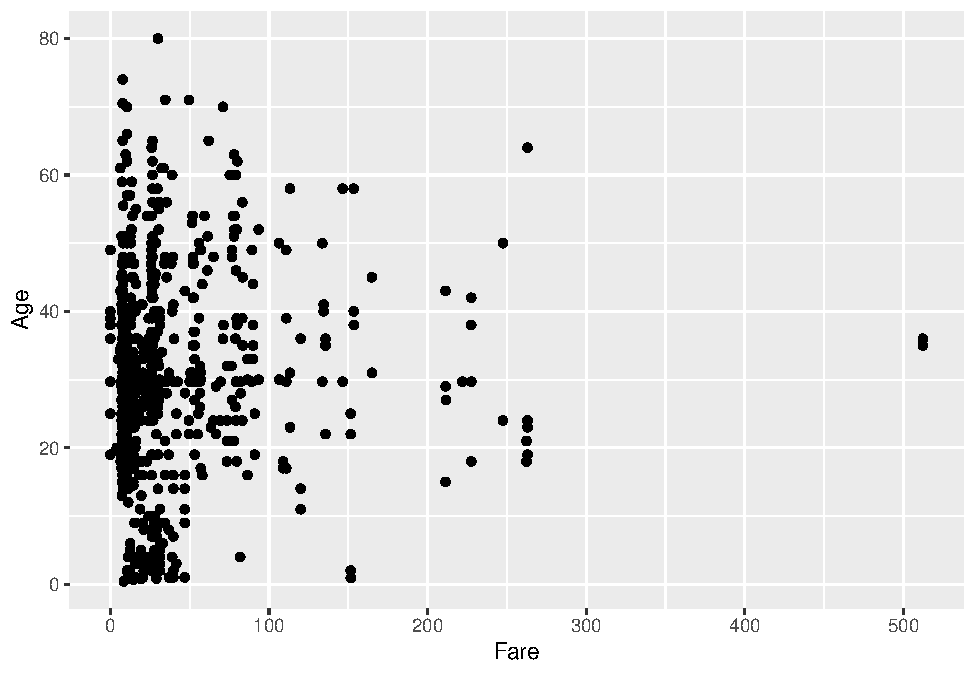
\includegraphics{Titanic-Documentation_files/figure-latex/unnamed-chunk-24-1.pdf}
According to the plot, we can say that the most paid fare ranges between
0-100 and the \textbf{age} between 15-50 had high numbers aboard. Two
outlers are detected at the far end of the \textbf{x-axis}, measures
should be carried inorder to decide on how to deal with them.

To check for the values we can do the following.

\begin{Shaded}
\begin{Highlighting}[]
\FunctionTok{filter\_all}\NormalTok{(titanic\_train\_data, }\FunctionTok{any\_vars}\NormalTok{(titanic\_train\_data}\SpecialCharTok{$}\NormalTok{Fare}\SpecialCharTok{\textgreater{}=}\DecValTok{500}\NormalTok{))}
\end{Highlighting}
\end{Shaded}

\begin{verbatim}
##   PassengerId Survived Pclass                               Name    Sex Age
## 1         259        1      1                   Ward, Miss. Anna female  35
## 2         680        1      1 Cardeza, Mr. Thomas Drake Martinez   male  36
## 3         738        1      1             Lesurer, Mr. Gustave J   male  35
##   SibSp Parch   Ticket     Fare       Cabin Embarked Age   Age       Age
## 1     0     0 PC 17755 512.3292                    C   2 youth non-child
## 2     0     1 PC 17755 512.3292 B51 B53 B55        C   3 adult non-child
## 3     0     0 PC 17755 512.3292        B101        C   2 youth non-child
\end{verbatim}

You will notice that they are three points with the same fare of
512.3292, embarked destination(c), Pclass(1) and ticket number(PC
17755).

\begin{Shaded}
\begin{Highlighting}[]
\NormalTok{titanic\_train\_data }\SpecialCharTok{\%\textgreater{}\%}
  \FunctionTok{select}\NormalTok{(Survived, Pclass,, Fare, Ticket ,age\_groups, Sex,Age) }\SpecialCharTok{\%\textgreater{}\%}
  \FunctionTok{ggplot}\NormalTok{(}\AttributeTok{data=}\NormalTok{) }\SpecialCharTok{+} 
  \FunctionTok{geom\_point}\NormalTok{(}\AttributeTok{mapping =}  \FunctionTok{aes}\NormalTok{(}\AttributeTok{x=}\NormalTok{Fare, }\AttributeTok{y=}\NormalTok{ Pclass), }\AttributeTok{stat =} \StringTok{"identity"}\NormalTok{)}
\end{Highlighting}
\end{Shaded}

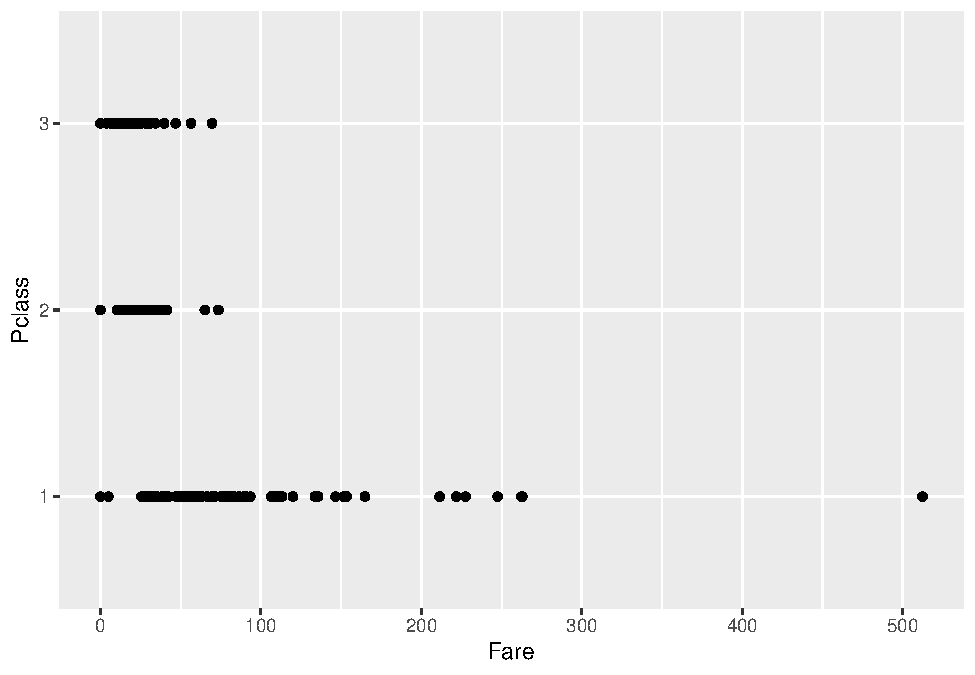
\includegraphics{Titanic-Documentation_files/figure-latex/unnamed-chunk-26-1.pdf}
Further investigation can be done as we see people in different
\textbf{Pclasses} paying the same fare.

\begin{Shaded}
\begin{Highlighting}[]
\FunctionTok{filter\_all}\NormalTok{(titanic\_train\_data, }\FunctionTok{any\_vars}\NormalTok{(titanic\_train\_data}\SpecialCharTok{$}\NormalTok{Pclass}\SpecialCharTok{==}\DecValTok{1} \SpecialCharTok{\&}\NormalTok{ titanic\_train\_data}\SpecialCharTok{$}\NormalTok{Fare}\SpecialCharTok{\textless{}}\DecValTok{500}\NormalTok{)) }\SpecialCharTok{\%\textgreater{}\%}
  \FunctionTok{head}\NormalTok{()}
\end{Highlighting}
\end{Shaded}

\begin{verbatim}
##   PassengerId Survived Pclass
## 1           2        1      1
## 2           4        1      1
## 3           7        0      1
## 4          12        1      1
## 5          24        1      1
## 6          28        0      1
##                                                  Name    Sex Age SibSp Parch
## 1 Cumings, Mrs. John Bradley (Florence Briggs Thayer) female  38     1     0
## 2        Futrelle, Mrs. Jacques Heath (Lily May Peel) female  35     1     0
## 3                             McCarthy, Mr. Timothy J   male  54     0     0
## 4                            Bonnell, Miss. Elizabeth female  58     0     0
## 5                        Sloper, Mr. William Thompson   male  28     0     0
## 6                      Fortune, Mr. Charles Alexander   male  19     3     2
##     Ticket     Fare       Cabin Embarked Age   Age       Age
## 1 PC 17599  71.2833         C85        C   3 adult non-child
## 2   113803  53.1000        C123        S   2 youth non-child
## 3    17463  51.8625         E46        S   3 adult non-child
## 4   113783  26.5500        C103        S   3 adult non-child
## 5   113788  35.5000          A6        S   2 youth non-child
## 6    19950 263.0000 C23 C25 C27        S   2 youth non-child
\end{verbatim}

\begin{Shaded}
\begin{Highlighting}[]
\NormalTok{titanic\_train\_data }\SpecialCharTok{\%\textgreater{}\%}
  \FunctionTok{select}\NormalTok{(Survived, Embarked, Pclass, Fare, Ticket ,age\_groups, Sex,Age) }\SpecialCharTok{\%\textgreater{}\%}
  \FunctionTok{ggplot}\NormalTok{(}\AttributeTok{data=}\NormalTok{) }\SpecialCharTok{+} 
  \FunctionTok{geom\_point}\NormalTok{(}\AttributeTok{mapping =}  \FunctionTok{aes}\NormalTok{(}\AttributeTok{x=}\NormalTok{Pclass, }\AttributeTok{y =}\NormalTok{ Fare), }\AttributeTok{stat =} \StringTok{"identity"}\NormalTok{) }\SpecialCharTok{+}
  \FunctionTok{facet\_grid}\NormalTok{( Embarked }\SpecialCharTok{\textasciitilde{}}\NormalTok{ Sex)}
\end{Highlighting}
\end{Shaded}

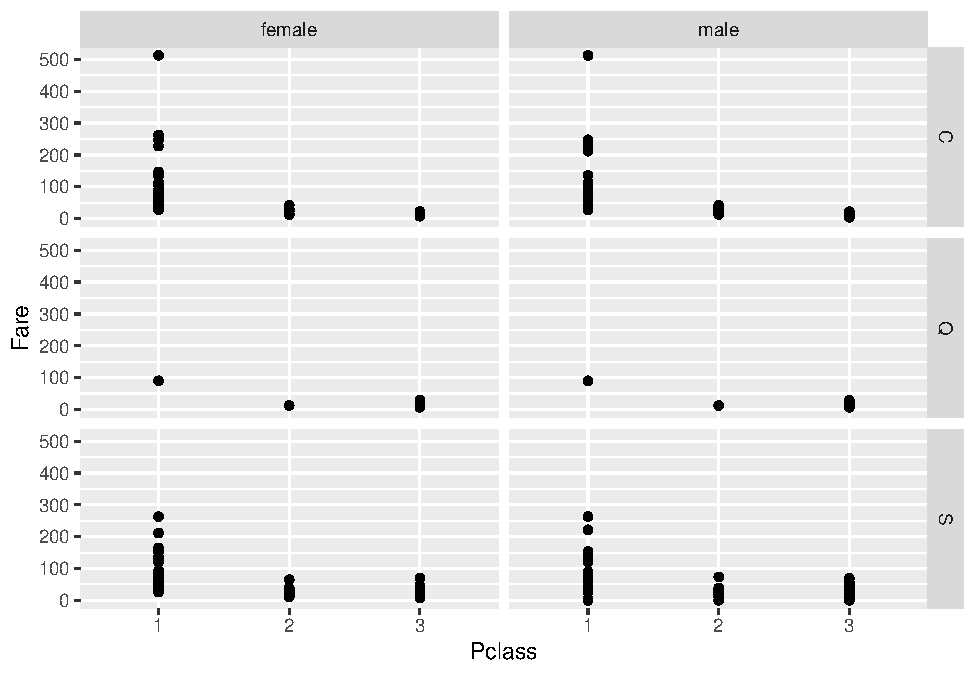
\includegraphics{Titanic-Documentation_files/figure-latex/unnamed-chunk-28-1.pdf}

\begin{Shaded}
\begin{Highlighting}[]
\NormalTok{titanic\_train\_data }\SpecialCharTok{\%\textgreater{}\%}
  \FunctionTok{select}\NormalTok{(Survived, Embarked, Pclass, age\_groups, Sex,Age) }\SpecialCharTok{\%\textgreater{}\%}
  \FunctionTok{ggplot}\NormalTok{(}\AttributeTok{data=}\NormalTok{) }\SpecialCharTok{+} 
  \FunctionTok{geom\_bar}\NormalTok{(}\AttributeTok{mapping =}  \FunctionTok{aes}\NormalTok{(}\AttributeTok{x=}\NormalTok{Embarked, }\AttributeTok{fill=} \FunctionTok{factor}\NormalTok{(Survived)), }\AttributeTok{color =} \StringTok{"black"}\NormalTok{, }\AttributeTok{position =} \FunctionTok{position\_dodge}\NormalTok{())}
\end{Highlighting}
\end{Shaded}

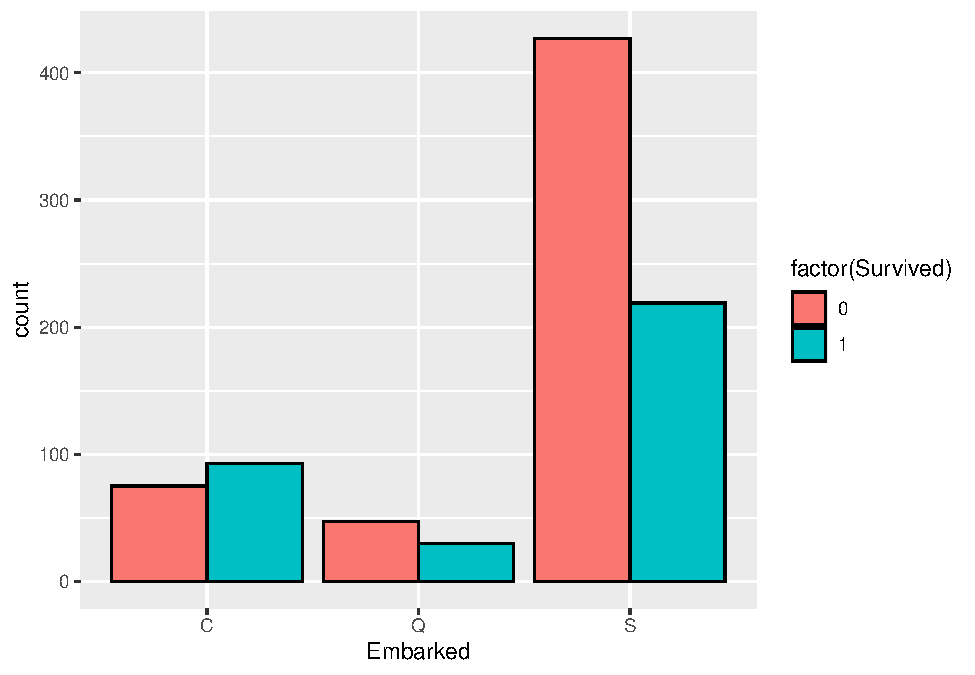
\includegraphics{Titanic-Documentation_files/figure-latex/unnamed-chunk-29-1.pdf}

\begin{Shaded}
\begin{Highlighting}[]
\NormalTok{titanic\_train\_data }\SpecialCharTok{\%\textgreater{}\%}
  \FunctionTok{select}\NormalTok{(Survived, Embarked, Pclass, age\_groups, Sex,Age) }\SpecialCharTok{\%\textgreater{}\%}
  \FunctionTok{ggplot}\NormalTok{(}\AttributeTok{data=}\NormalTok{) }\SpecialCharTok{+} 
  \FunctionTok{geom\_bar}\NormalTok{(}\AttributeTok{mapping =}  \FunctionTok{aes}\NormalTok{(}\AttributeTok{x=}\NormalTok{Sex, }\AttributeTok{fill=} \FunctionTok{factor}\NormalTok{(Survived)), }\AttributeTok{color =} \StringTok{"black"}\NormalTok{, }\AttributeTok{position =} \FunctionTok{position\_dodge}\NormalTok{())}
\end{Highlighting}
\end{Shaded}

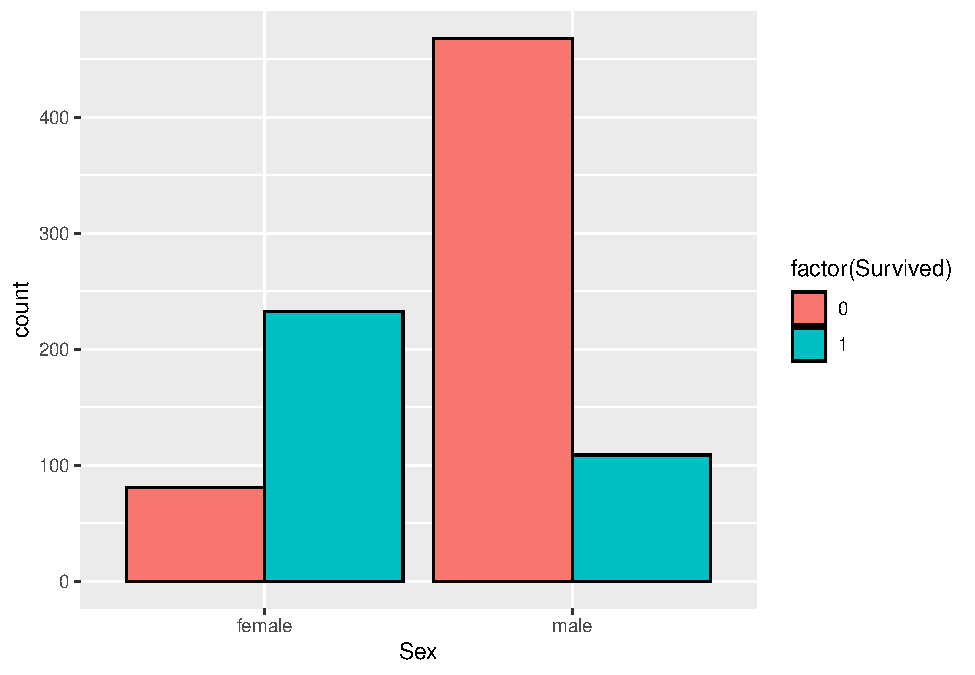
\includegraphics{Titanic-Documentation_files/figure-latex/unnamed-chunk-30-1.pdf}

\begin{Shaded}
\begin{Highlighting}[]
\NormalTok{titanic\_train\_data }\SpecialCharTok{\%\textgreater{}\%}
  \FunctionTok{select}\NormalTok{(Survived,SibSp) }\SpecialCharTok{\%\textgreater{}\%}
  \FunctionTok{ggplot}\NormalTok{(}\AttributeTok{data=}\NormalTok{) }\SpecialCharTok{+} 
  \FunctionTok{geom\_bar}\NormalTok{(}\AttributeTok{mapping =}  \FunctionTok{aes}\NormalTok{(}\AttributeTok{x=}\NormalTok{SibSp, }\AttributeTok{fill=} \FunctionTok{factor}\NormalTok{(Survived)), }\AttributeTok{color =} \StringTok{"black"}\NormalTok{, }\AttributeTok{position =} \FunctionTok{position\_dodge}\NormalTok{())}
\end{Highlighting}
\end{Shaded}

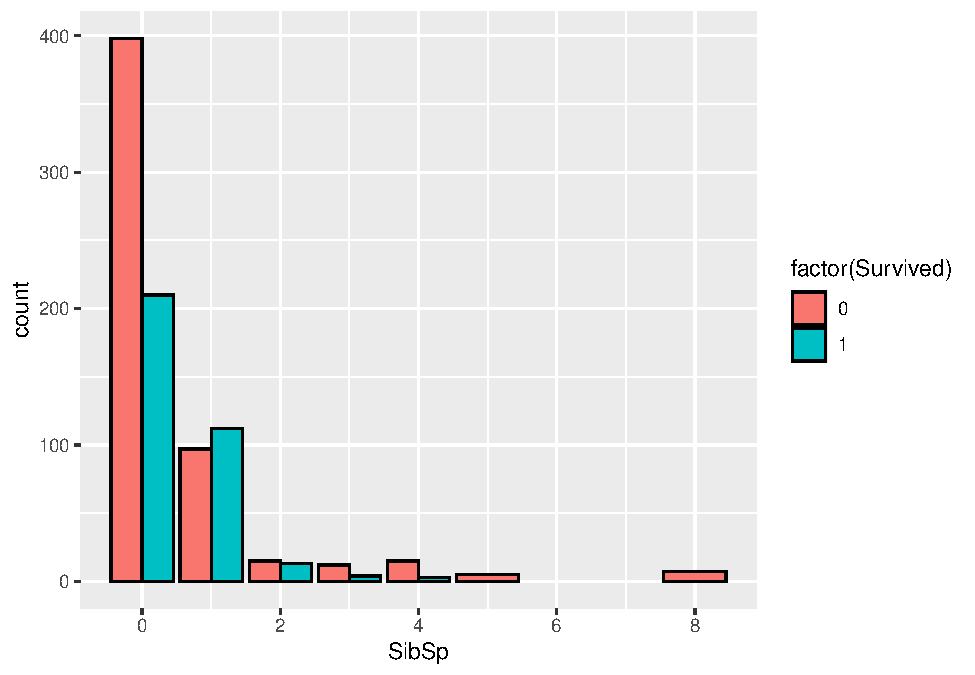
\includegraphics{Titanic-Documentation_files/figure-latex/unnamed-chunk-31-1.pdf}

\begin{Shaded}
\begin{Highlighting}[]
\NormalTok{titanic\_train\_data }\SpecialCharTok{\%\textgreater{}\%}
  \FunctionTok{select}\NormalTok{(Survived, SibSp, Sex, age\_groups) }\SpecialCharTok{\%\textgreater{}\%}
  \FunctionTok{ggplot}\NormalTok{(}\AttributeTok{data=}\NormalTok{) }\SpecialCharTok{+} 
  \FunctionTok{geom\_bar}\NormalTok{(}\AttributeTok{mapping =}  \FunctionTok{aes}\NormalTok{(}\AttributeTok{x=}\NormalTok{SibSp, }\AttributeTok{fill=} \FunctionTok{factor}\NormalTok{(Survived)), }\AttributeTok{color =} \StringTok{"black"}\NormalTok{, }\AttributeTok{position =} \FunctionTok{position\_dodge}\NormalTok{()) }\SpecialCharTok{+}
  \FunctionTok{facet\_grid}\NormalTok{(Sex}\SpecialCharTok{\textasciitilde{}}\NormalTok{age\_groups)}
\end{Highlighting}
\end{Shaded}

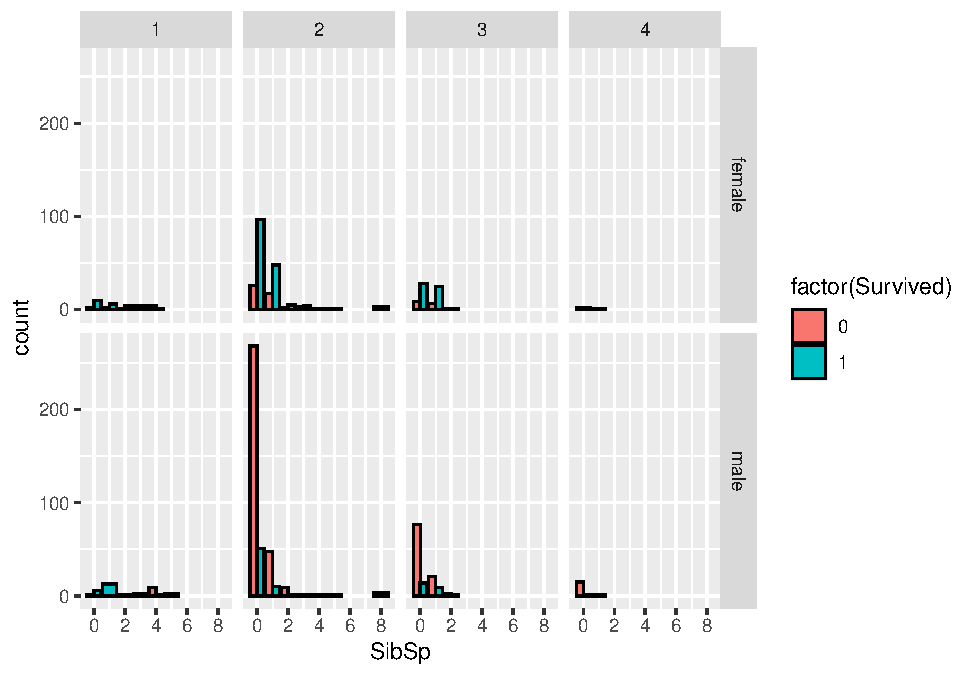
\includegraphics{Titanic-Documentation_files/figure-latex/unnamed-chunk-32-1.pdf}

\begin{Shaded}
\begin{Highlighting}[]
\NormalTok{titanic\_train\_data }\SpecialCharTok{\%\textgreater{}\%}
  \FunctionTok{select}\NormalTok{(Survived, Parch) }\SpecialCharTok{\%\textgreater{}\%}
  \FunctionTok{ggplot}\NormalTok{(}\AttributeTok{data=}\NormalTok{) }\SpecialCharTok{+} 
  \FunctionTok{geom\_bar}\NormalTok{(}\AttributeTok{mapping =}  \FunctionTok{aes}\NormalTok{(}\AttributeTok{x=}\NormalTok{Parch, }\AttributeTok{fill=} \FunctionTok{factor}\NormalTok{(Survived)), }\AttributeTok{color =} \StringTok{"black"}\NormalTok{, }\AttributeTok{position =} \FunctionTok{position\_dodge}\NormalTok{())}
\end{Highlighting}
\end{Shaded}

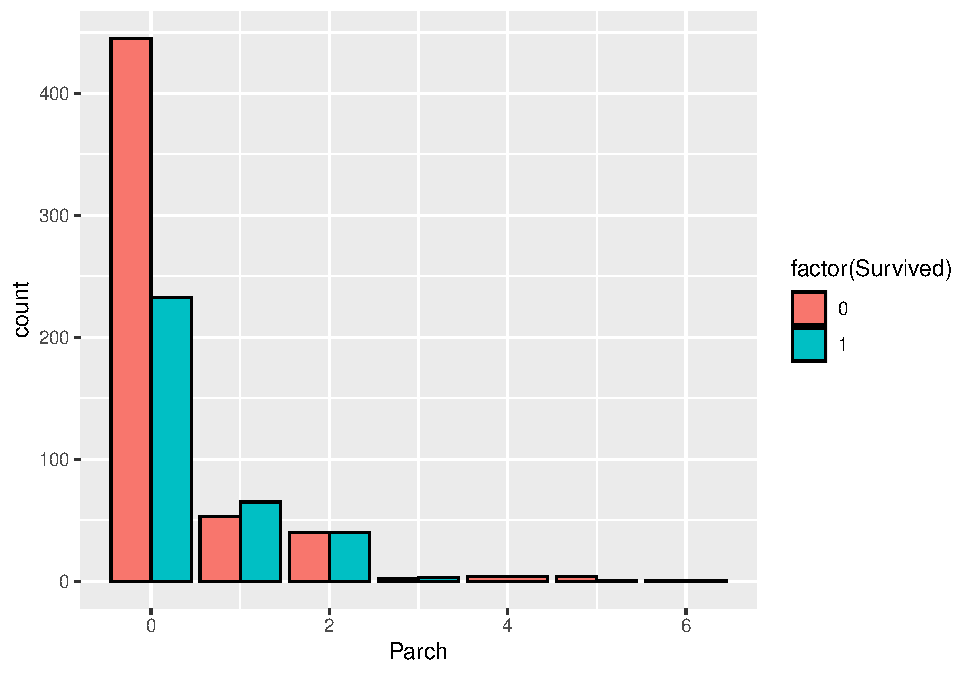
\includegraphics{Titanic-Documentation_files/figure-latex/unnamed-chunk-33-1.pdf}

\begin{Shaded}
\begin{Highlighting}[]
\NormalTok{titanic\_train\_data }\SpecialCharTok{\%\textgreater{}\%}
  \FunctionTok{select}\NormalTok{(Survived, Parch, Sex, age\_groups) }\SpecialCharTok{\%\textgreater{}\%}
  \FunctionTok{ggplot}\NormalTok{(}\AttributeTok{data=}\NormalTok{) }\SpecialCharTok{+} 
  \FunctionTok{geom\_bar}\NormalTok{(}\AttributeTok{mapping =}  \FunctionTok{aes}\NormalTok{(}\AttributeTok{x=}\NormalTok{Parch, }\AttributeTok{fill=} \FunctionTok{factor}\NormalTok{(Survived)), }\AttributeTok{color =} \StringTok{"black"}\NormalTok{, }\AttributeTok{position =} \FunctionTok{position\_dodge}\NormalTok{()) }\SpecialCharTok{+}
  \FunctionTok{facet\_grid}\NormalTok{(Sex}\SpecialCharTok{\textasciitilde{}}\NormalTok{age\_groups)}
\end{Highlighting}
\end{Shaded}

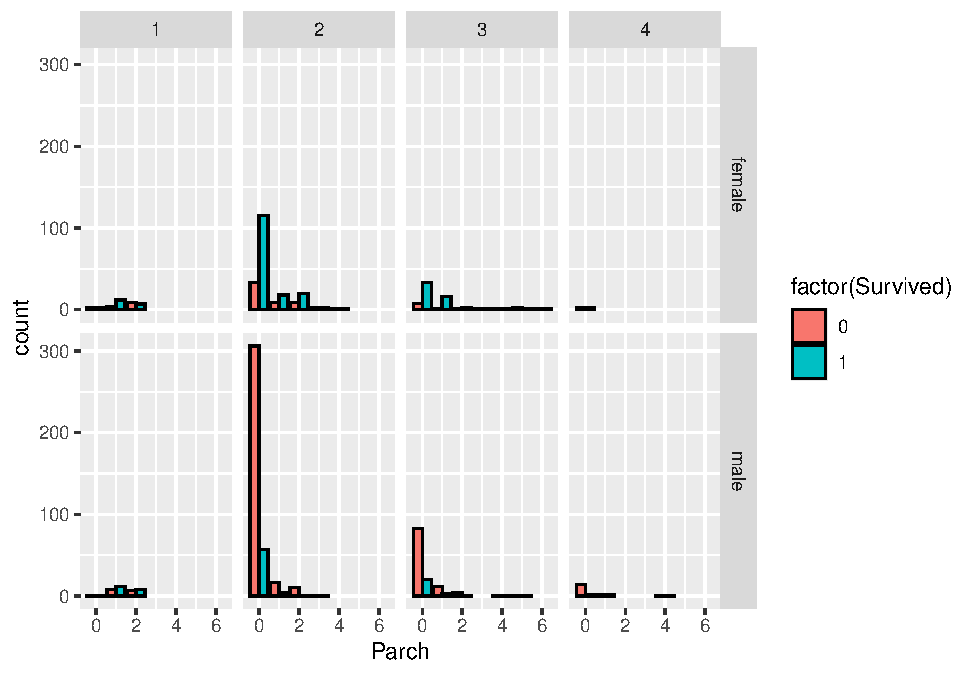
\includegraphics{Titanic-Documentation_files/figure-latex/unnamed-chunk-34-1.pdf}

\begin{Shaded}
\begin{Highlighting}[]
\NormalTok{titanic\_train\_data }\SpecialCharTok{\%\textgreater{}\%}
  \FunctionTok{select}\NormalTok{(Survived, Pclass, age\_groups, Sex,Age) }\SpecialCharTok{\%\textgreater{}\%}
  \FunctionTok{ggplot}\NormalTok{(}\AttributeTok{data=}\NormalTok{) }\SpecialCharTok{+} 
  \FunctionTok{geom\_bar}\NormalTok{(}\AttributeTok{mapping =}  \FunctionTok{aes}\NormalTok{(}\AttributeTok{x=}\NormalTok{Pclass, }\AttributeTok{fill=} \FunctionTok{factor}\NormalTok{(Survived)), }\AttributeTok{color =} \StringTok{"black"}\NormalTok{, }\AttributeTok{position =} \FunctionTok{position\_dodge}\NormalTok{()) }\SpecialCharTok{+}
  \FunctionTok{facet\_grid}\NormalTok{(Sex }\SpecialCharTok{\textasciitilde{}}\NormalTok{ age\_groups)}
\end{Highlighting}
\end{Shaded}

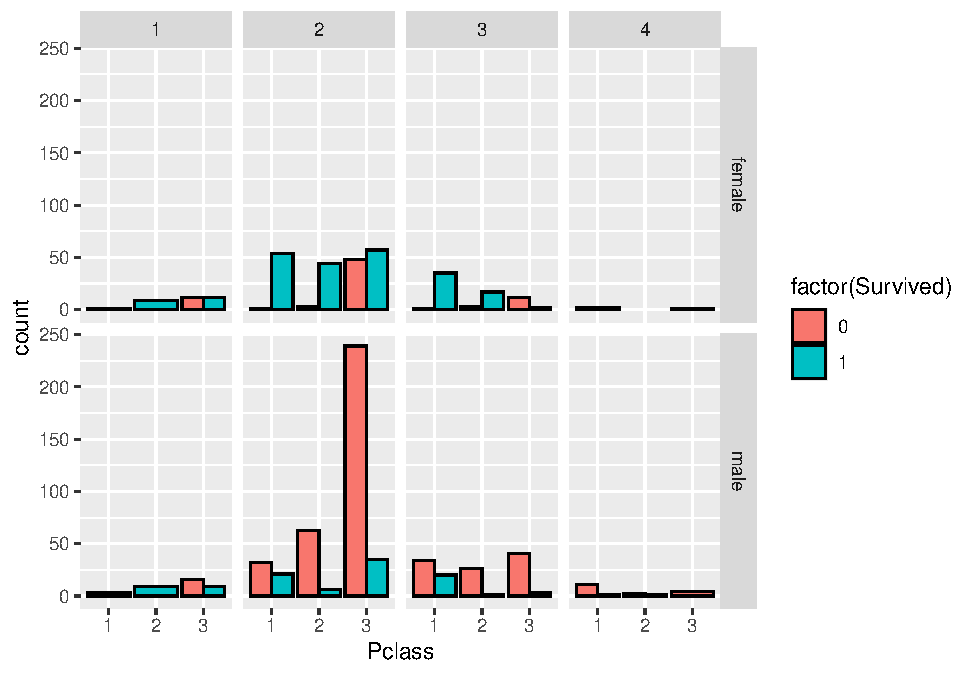
\includegraphics{Titanic-Documentation_files/figure-latex/unnamed-chunk-35-1.pdf}

\begin{Shaded}
\begin{Highlighting}[]
\NormalTok{titanic\_train\_data }\SpecialCharTok{\%\textgreater{}\%}
  \FunctionTok{select}\NormalTok{(Survived, Pclass, age\_groups, Sex,Age) }\SpecialCharTok{\%\textgreater{}\%}
  \FunctionTok{ggplot}\NormalTok{(}\AttributeTok{data=}\NormalTok{) }\SpecialCharTok{+} 
  \FunctionTok{geom\_bar}\NormalTok{(}\AttributeTok{mapping =}  \FunctionTok{aes}\NormalTok{(}\AttributeTok{x=}\FunctionTok{factor}\NormalTok{(Pclass), }\AttributeTok{y =}\NormalTok{ Age, }\AttributeTok{fill=}\NormalTok{ Survived), }\AttributeTok{stat =} \StringTok{"identity"}\NormalTok{,  }\AttributeTok{position=}\FunctionTok{position\_dodge}\NormalTok{())}
\end{Highlighting}
\end{Shaded}

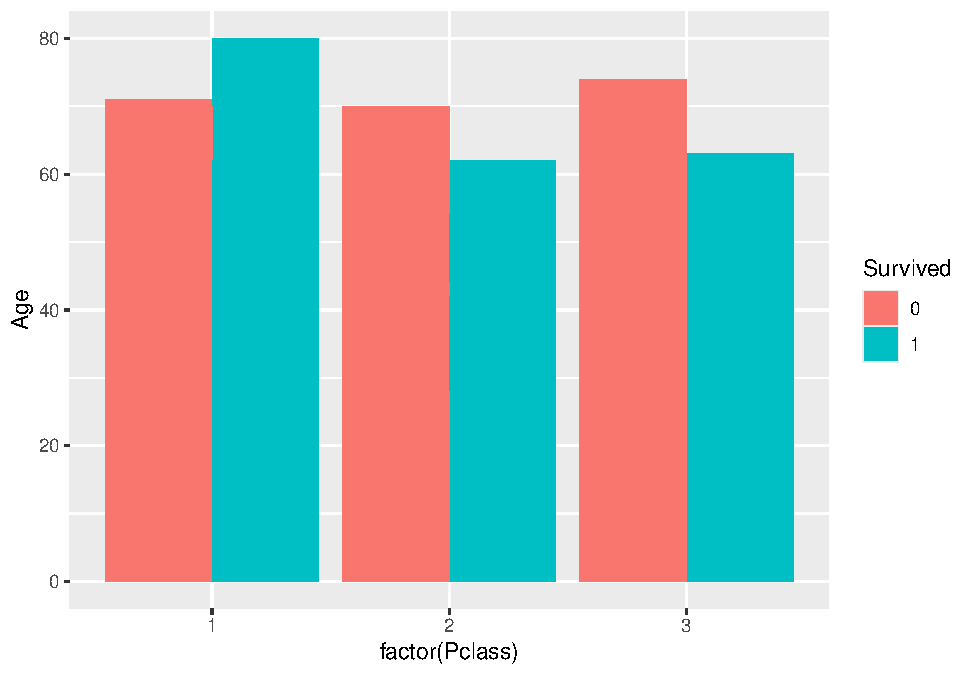
\includegraphics{Titanic-Documentation_files/figure-latex/unnamed-chunk-36-1.pdf}

\begin{Shaded}
\begin{Highlighting}[]
\NormalTok{titanic\_train\_data }\SpecialCharTok{\%\textgreater{}\%}
  \FunctionTok{select}\NormalTok{(Survived, Pclass, age\_groups, Sex,Age) }\SpecialCharTok{\%\textgreater{}\%}
  \FunctionTok{ggplot}\NormalTok{(}\AttributeTok{data=}\NormalTok{) }\SpecialCharTok{+} 
  \FunctionTok{geom\_bar}\NormalTok{(}\AttributeTok{mapping =}  \FunctionTok{aes}\NormalTok{(}\AttributeTok{x=}\NormalTok{Pclass, }\AttributeTok{y =}\NormalTok{ Age, }\AttributeTok{fill=} \FunctionTok{factor}\NormalTok{(Survived)), }\AttributeTok{stat =} \StringTok{"identity"}\NormalTok{,  }\AttributeTok{position=}\FunctionTok{position\_dodge}\NormalTok{()) }\SpecialCharTok{+}
  \FunctionTok{facet\_grid}\NormalTok{(Sex }\SpecialCharTok{\textasciitilde{}}\NormalTok{ age\_groups)}
\end{Highlighting}
\end{Shaded}

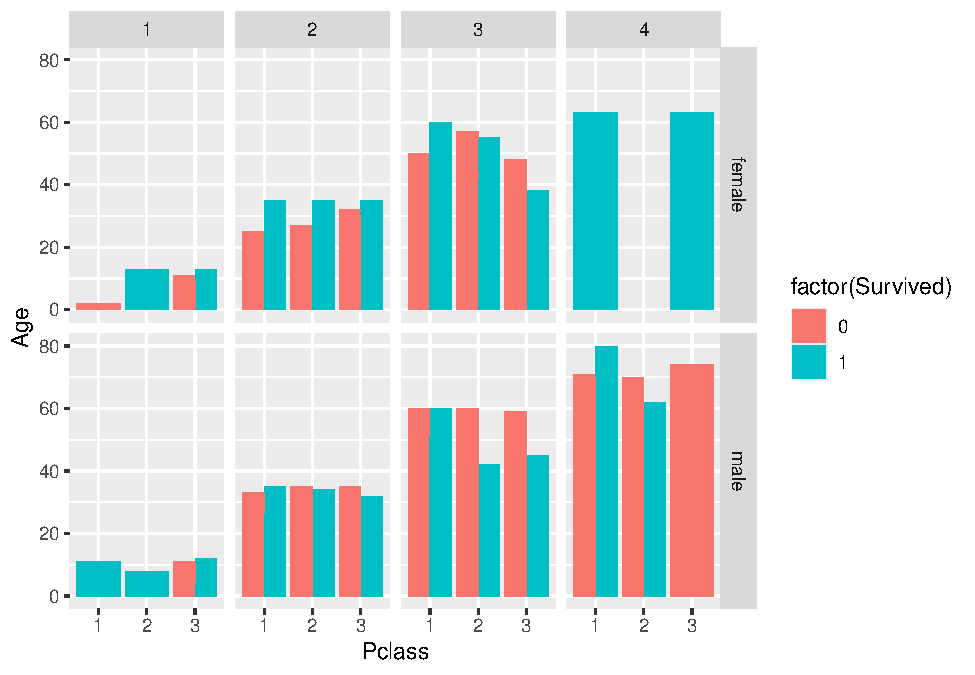
\includegraphics{Titanic-Documentation_files/figure-latex/unnamed-chunk-37-1.pdf}

\begin{Shaded}
\begin{Highlighting}[]
\CommentTok{\#setting factors to categorical data}
\NormalTok{titanic\_test\_data}\SpecialCharTok{$}\NormalTok{Survived }\OtherTok{\textless{}{-}} \ConstantTok{NA}
\NormalTok{titanic\_test\_data}\SpecialCharTok{$}\NormalTok{Survived}\OtherTok{\textless{}{-}} \FunctionTok{as.factor}\NormalTok{(titanic\_test\_data}\SpecialCharTok{$}\NormalTok{Survived)}
\end{Highlighting}
\end{Shaded}

\hypertarget{modelling-the-data.}{%
\subsection{Modelling the data.}\label{modelling-the-data.}}

\hypertarget{method-one-for-doing-our-prediction}{%
\subsubsection{Method one for doing our
prediction}\label{method-one-for-doing-our-prediction}}

\begin{Shaded}
\begin{Highlighting}[]
\NormalTok{rf.model}\OtherTok{\textless{}{-}}\FunctionTok{randomForest}\NormalTok{(}\FunctionTok{factor}\NormalTok{(Survived) }\SpecialCharTok{\textasciitilde{}}\NormalTok{  age\_groups }\SpecialCharTok{+}\NormalTok{ SibSp }\SpecialCharTok{+}\NormalTok{ Parch }\SpecialCharTok{+}\NormalTok{ Sex }\SpecialCharTok{+}\NormalTok{ Pclass }\SpecialCharTok{+}\NormalTok{ Embarked, }\AttributeTok{data=}\NormalTok{ titanic\_train\_data)}
\NormalTok{rf.model }\SpecialCharTok{\%\textgreater{}\%}
  \FunctionTok{predict}\NormalTok{() }\SpecialCharTok{\%\textgreater{}\%}
  \FunctionTok{table}\NormalTok{()}
\end{Highlighting}
\end{Shaded}

\begin{verbatim}
## .
##   0   1 
## 626 265
\end{verbatim}

\hypertarget{method-two-for-doing-our-prediction.}{%
\subsubsection{Method two for doing our
prediction.}\label{method-two-for-doing-our-prediction.}}

\begin{Shaded}
\begin{Highlighting}[]
\NormalTok{titanic\_train\_data}\SpecialCharTok{$}\NormalTok{Age}\OtherTok{\textless{}{-}}\NormalTok{ titanic\_train\_data}\SpecialCharTok{\%\textgreater{}\%}
  \FunctionTok{select}\NormalTok{(Age) }\SpecialCharTok{\%\textgreater{}\%}
  \FunctionTok{apply}\NormalTok{(}\FunctionTok{c}\NormalTok{(}\DecValTok{2}\NormalTok{), . }\SpecialCharTok{\%\textgreater{}\%}\NormalTok{ \{}\FunctionTok{ifelse}\NormalTok{(}\FunctionTok{is.na}\NormalTok{(.), }\FloatTok{29.70}\NormalTok{, .)\})}

\NormalTok{titanic\_train\_data.head }\OtherTok{\textless{}{-}}\NormalTok{ titanic\_train\_data}

\NormalTok{titanic\_test\_data.head }\OtherTok{\textless{}{-}}\NormalTok{ titanic\_train\_data }\SpecialCharTok{\%\textgreater{}\%}
  \FunctionTok{mutate}\NormalTok{(}\AttributeTok{Age =} \ConstantTok{NA}\NormalTok{)}

\FunctionTok{str}\NormalTok{(titanic\_test\_data.head)}
\end{Highlighting}
\end{Shaded}

\begin{verbatim}
## 'data.frame':    891 obs. of  15 variables:
##  $ PassengerId        : int  1 2 3 4 5 6 7 8 9 10 ...
##  $ Survived           : Factor w/ 2 levels "0","1": 1 2 2 2 1 1 1 1 2 2 ...
##  $ Pclass             : Factor w/ 3 levels "1","2","3": 3 1 3 1 3 3 1 3 3 2 ...
##  $ Name               : chr  "Braund, Mr. Owen Harris" "Cumings, Mrs. John Bradley (Florence Briggs Thayer)" "Heikkinen, Miss. Laina" "Futrelle, Mrs. Jacques Heath (Lily May Peel)" ...
##  $ Sex                : Factor w/ 2 levels "female","male": 2 1 1 1 2 2 2 2 1 1 ...
##  $ Age                : logi  NA NA NA NA NA NA ...
##  $ SibSp              : int  1 1 0 1 0 0 0 3 0 1 ...
##  $ Parch              : int  0 0 0 0 0 0 0 1 2 0 ...
##  $ Ticket             : chr  "A/5 21171" "PC 17599" "STON/O2. 3101282" "113803" ...
##  $ Fare               : num  7.25 71.28 7.92 53.1 8.05 ...
##  $ Cabin              : chr  "" "C85" "" "C123" ...
##  $ Embarked           : Factor w/ 4 levels "","C","Q","S": 4 2 4 4 4 3 4 4 4 2 ...
##  $ age_groups         : num [1:891, 1] 2 3 2 2 2 2 3 1 2 2 ...
##   ..- attr(*, "dimnames")=List of 2
##   .. ..$ : NULL
##   .. ..$ : chr "Age"
##  $ age_groups_young   : chr [1:891, 1] "youth" "adult" "youth" "youth" ...
##   ..- attr(*, "dimnames")=List of 2
##   .. ..$ : NULL
##   .. ..$ : chr "Age"
##  $ age_groups_children: chr [1:891, 1] "non-child" "non-child" "non-child" "non-child" ...
##   ..- attr(*, "dimnames")=List of 2
##   .. ..$ : NULL
##   .. ..$ : chr "Age"
\end{verbatim}

\begin{Shaded}
\begin{Highlighting}[]
\FunctionTok{str}\NormalTok{(titanic\_train\_data.head)}
\end{Highlighting}
\end{Shaded}

\begin{verbatim}
## 'data.frame':    891 obs. of  15 variables:
##  $ PassengerId        : int  1 2 3 4 5 6 7 8 9 10 ...
##  $ Survived           : Factor w/ 2 levels "0","1": 1 2 2 2 1 1 1 1 2 2 ...
##  $ Pclass             : Factor w/ 3 levels "1","2","3": 3 1 3 1 3 3 1 3 3 2 ...
##  $ Name               : chr  "Braund, Mr. Owen Harris" "Cumings, Mrs. John Bradley (Florence Briggs Thayer)" "Heikkinen, Miss. Laina" "Futrelle, Mrs. Jacques Heath (Lily May Peel)" ...
##  $ Sex                : Factor w/ 2 levels "female","male": 2 1 1 1 2 2 2 2 1 1 ...
##  $ Age                : num [1:891, 1] 22 38 26 35 35 ...
##   ..- attr(*, "dimnames")=List of 2
##   .. ..$ : NULL
##   .. ..$ : chr "Age"
##  $ SibSp              : int  1 1 0 1 0 0 0 3 0 1 ...
##  $ Parch              : int  0 0 0 0 0 0 0 1 2 0 ...
##  $ Ticket             : chr  "A/5 21171" "PC 17599" "STON/O2. 3101282" "113803" ...
##  $ Fare               : num  7.25 71.28 7.92 53.1 8.05 ...
##  $ Cabin              : chr  "" "C85" "" "C123" ...
##  $ Embarked           : Factor w/ 4 levels "","C","Q","S": 4 2 4 4 4 3 4 4 4 2 ...
##  $ age_groups         : num [1:891, 1] 2 3 2 2 2 2 3 1 2 2 ...
##   ..- attr(*, "dimnames")=List of 2
##   .. ..$ : NULL
##   .. ..$ : chr "Age"
##  $ age_groups_young   : chr [1:891, 1] "youth" "adult" "youth" "youth" ...
##   ..- attr(*, "dimnames")=List of 2
##   .. ..$ : NULL
##   .. ..$ : chr "Age"
##  $ age_groups_children: chr [1:891, 1] "non-child" "non-child" "non-child" "non-child" ...
##   ..- attr(*, "dimnames")=List of 2
##   .. ..$ : NULL
##   .. ..$ : chr "Age"
\end{verbatim}

\begin{Shaded}
\begin{Highlighting}[]
\NormalTok{modeleAge}\OtherTok{\textless{}{-}}\NormalTok{titanic\_train\_data.head }\SpecialCharTok{\%\textgreater{}\%}
  \FunctionTok{select}\NormalTok{(Age, Fare, Parch, Survived, SibSp, Pclass, Ticket, Sex) }\SpecialCharTok{\%\textgreater{}\%}
  \FunctionTok{lm}\NormalTok{(Age }\SpecialCharTok{\textasciitilde{}}\NormalTok{ Fare }\SpecialCharTok{+}\NormalTok{ Parch }\SpecialCharTok{+}\NormalTok{ Survived }\SpecialCharTok{+}\NormalTok{ SibSp }\SpecialCharTok{+}\NormalTok{ Pclass }\SpecialCharTok{+}\NormalTok{ Ticket }\SpecialCharTok{+}\NormalTok{Sex, }\AttributeTok{data=}\NormalTok{ .) }

\NormalTok{predicted.Age}\OtherTok{\textless{}{-}} \FunctionTok{predict}\NormalTok{(modeleAge , }\AttributeTok{newdata =}\NormalTok{  titanic\_test\_data.head) }
\end{Highlighting}
\end{Shaded}

\begin{verbatim}
## Warning in predict.lm(modeleAge, newdata = titanic_test_data.head): prediction
## from a rank-deficient fit may be misleading
\end{verbatim}

\begin{Shaded}
\begin{Highlighting}[]
\NormalTok{titanic\_train\_data}\SpecialCharTok{$}\NormalTok{Age}\OtherTok{\textless{}{-}}\NormalTok{ predicted.Age}

\NormalTok{Model.Survive}\OtherTok{\textless{}{-}}\FunctionTok{randomForest}\NormalTok{(Survived }\SpecialCharTok{\textasciitilde{}}\NormalTok{ Age }\SpecialCharTok{+}\NormalTok{  SibSp }\SpecialCharTok{+}\NormalTok{ Parch }\SpecialCharTok{+}\NormalTok{ Sex }\SpecialCharTok{+}\NormalTok{ Pclass }\SpecialCharTok{+}\NormalTok{ Embarked }\SpecialCharTok{+}\NormalTok{ Fare, }\AttributeTok{data=}\NormalTok{ titanic\_train\_data) }

\NormalTok{Model.Survive }\SpecialCharTok{\%\textgreater{}\%}
  \FunctionTok{predict}\NormalTok{() }\SpecialCharTok{\%\textgreater{}\%}
  \FunctionTok{table}\NormalTok{()}
\end{Highlighting}
\end{Shaded}

\begin{verbatim}
## .
##   0   1 
## 609 282
\end{verbatim}

\begin{Shaded}
\begin{Highlighting}[]
\NormalTok{rf.Predicted.Survive}\OtherTok{\textless{}{-}}\NormalTok{rf.model }\SpecialCharTok{\%\textgreater{}\%}
  \FunctionTok{predict}\NormalTok{()}
\NormalTok{rf.Predicted.Survive.table}\OtherTok{\textless{}{-}}\FunctionTok{as.data.frame}\NormalTok{(rf.Predicted.Survive)}
\end{Highlighting}
\end{Shaded}


\end{document}
